\clearpage{}

\section{Describe elements of project schedules: work breakdown structure,
tasks, deliverables and milestones. Explain the critical path method.
Illustrate on PERT and Gantt charts. Discuss resource planning and
tracking.}

\subsection{Elements of project schedules}

A project can be divided into a list of tasks, each one subdivided into
sub-tasks. Therefore, scheduling a project consists of estimating the
\textbf{duration} and \textbf{resources} need

\begin{itemize}
	\item How \textit{long} will it take to develop the system?
	\item How \textit{much} will it cost to develop the system?
\end{itemize}

\subsubsection{Task (activity)}
A part of the project that takes place over a period of time.

\begin{itemize}
    \item \textbf{Predecessors (precursors):} events that must occur in order for a
    task to start
    \item \textbf{Duration:} length of time needed to complete a task.
    \item \textbf{Due date:} date by which a task must be completed.
    \item \textbf{Endpoint:} event marking the end of the task.
\end{itemize}

\subsubsection{Work breakdown structure}
A hierarchical decomposition of a project into tasks.
\begin{figure}[!ht]
    \centering
    \begin{tikzpicture}[node distance=0.5cm,on grid, auto]
[-,thick]
\footnotesize
\node[draw] {Build communications software} [edge from parent fork down]
  child {node[draw, left=0.5cm] {System planning (1.0)}
    child {node[draw] {Review specification (1.1)}
        child {node[draw] {Review budget (1.2)}
            child {node[draw] {Review schedule (1.3)}
                child {node[draw] {Develop plan (1.4)}}
            }
        }
    }
  }
  child {node[draw] {System design (2.0)}
    child {node[draw] {Top-level design (2.1)}
        child {node[draw] {Prototyping (2.2)}
            child {node[draw] {User interface (2.3)}
                child {node[draw] {Detailed design (2.4)}}
            }
        }
    }
  }
  child {node[draw, right=0.4cm] {Coding (3.0)}}
  child {node[draw, right=1cm] {Testing (4.0)}}
  child {node[draw, right=1.6cm] {Delivery (5.0)}};
\end{tikzpicture}

    \caption{Work breakdown structure}
\end{figure}



\subsubsection{Deliverable}
An item to be delivered to the customer (software, documents, technical demonstrations of a functionality, performance, reliability,...).

\subsubsection{Milestones}
A particular point in the progress of a project such as the completion of a task. It allows to pinpoint when the requirements specification are completed, or when the user manual has been delivered for example. Therefore, the delivery of a deliverable is a milestone.


\subsection{Critical Path Method (CPM)}

The CPM is an algorithm for scheduling a set of project activities.
\begin{itemize}
    \item shows us the \textbf{minimum amount of time} it will take to
        complete the project, given our estimates of each activity’s duration
        and predecessors.
    \item reveals the \textbf{most critical tasks} to complete
        the project on time (can be more than one)
\end{itemize}


Gantt and PERT chart are both appropriate to apply the algorithm because they contain all the
required information. Although, in my opinion, PERT is the best representation to apply the
algorithm and Gantt is better to show the plan resulting from the algorithm.

\subsubsection{Algorithm:}

\begin{figure}[!ht]
\begin{minipage}[t]{\linewidth}
    \begin{minipage}[c]{0.6\linewidth}
        \begin{lstlisting}[mathescape, frame=single, caption={CPM Algorithm},captionpos=b]
For each task $i$:
    duration $d_i$
    earliest start time $s_i$
    earliest end time $e_i$

Given all $d_i$, compute all $s_i$ and $e_i$
Start task: $s_{START} = 0, e_{START} = d_{START}$
For all tasks $i$ (in predecessor order):
    $s_i = \max \{e_j \mid j \textrm{ is a predecessor of } i\}$
    $e_i = s_i + d_i$
        \end{lstlisting}
    \end{minipage}
    \begin{minipage}[c]{0.35\linewidth}
        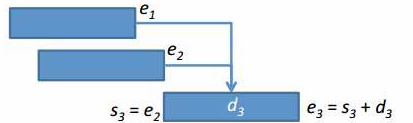
\includegraphics[width=\linewidth]{cpm_algorithm.png}
        \caption{CPM Algorithm}
    \end{minipage}
\end{minipage}
    \begin{minipage}{0.8\linewidth}
		\begin{lstlisting}[mathescape, frame=single, caption={CPM results}, captionpos=b]
Earliest project end time = $e_{FINISH}$
For each task $i$:
	latest end time $e_{i}'$ = min {$s_j \mid i$ is a predecessor of $j$}
	latest start time $s_{i}' = e_{i}' - d_i$
	available time $d_{i}' = e_{i}' - s_i$
	slack time (float) $f_i = e_{i}' - e_i = s_{i}' - s_i = d_{i}' - d_i$
		\end{lstlisting}
		\centering
    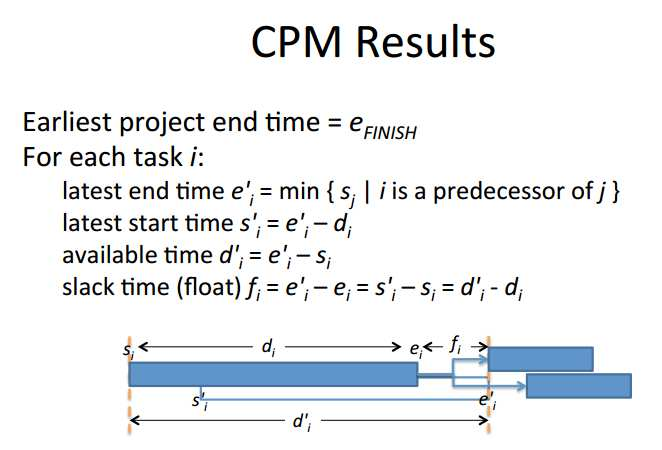
\includegraphics[width=0.6\linewidth]{cpm_results.png}
    \caption{CPM results}
	\end{minipage}
\end{figure}
\FloatBarrier{}

\subsubsection{PERT Chart}

The PERT chart is an activity graph that can be used to represent the
arrangement of the different tasks of the project and the relations
among them (predecessors, successors). Each node in the graph
corresponds to one task and is bound to an estimated duration time to
complete this task.

\begin{figure}[!ht]
    \centering
    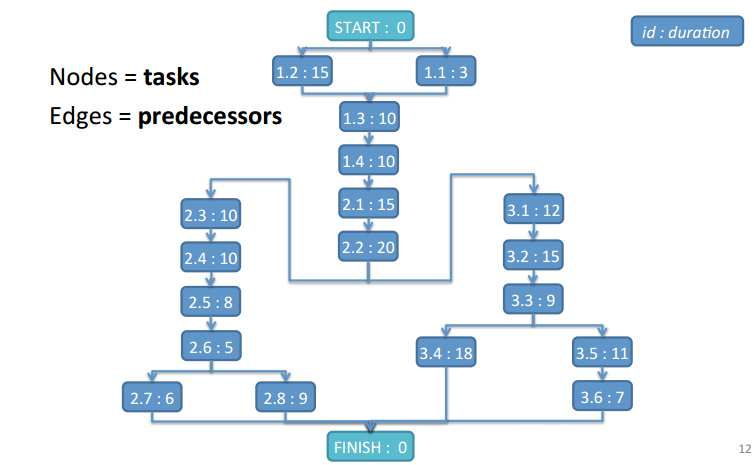
\includegraphics[width=0.5\linewidth]{pert_chart.png}
    \caption{PERT Chart}
\end{figure}
\FloatBarrier{}

\subsubsection{Gantt Chart}

The Gantt chart is another way to represent the arrangement of the
tasks. The X-axis represents the time and the y-axis the different tasks
to complete. (time duration) of the tasks.

\begin{figure}[!ht]
    \centering
    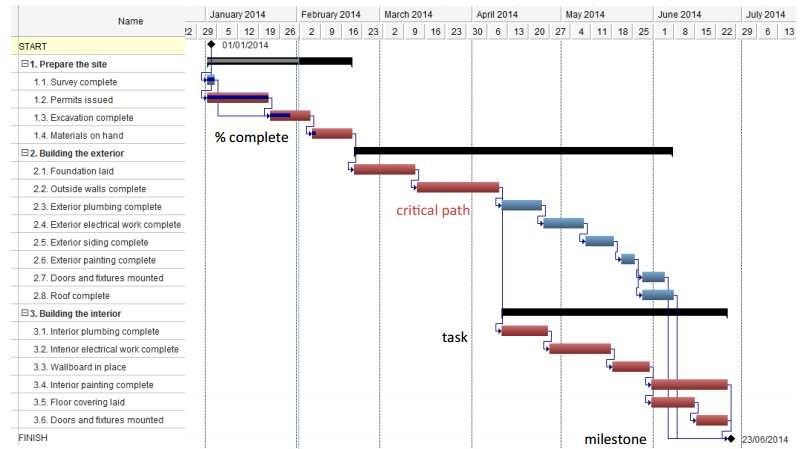
\includegraphics[width=0.5\linewidth]{gantt_chart.png}
    \caption{Gantt Chart}
\end{figure}
\FloatBarrier{}


\subsection{Resource planning and tracking}

\subsubsection{Resource planning}
Consists to estimate the resource usage for each task in terms of:
\begin{itemize}
    \item Staff [pers]
    \item Supplies [units/day]
    \item Expenditure [\$/day]
\end{itemize}

\begin{tabular}{m{8cm}m{9cm}}
    Guidelines: & Resource planning and tracking \\
    \begin{enumerate}
        \item Sum the resources required at each time for all task
        \item Compare to the available resources.
        \item Track actual vs.\ planned resource usage.
    \end{enumerate}
    &
    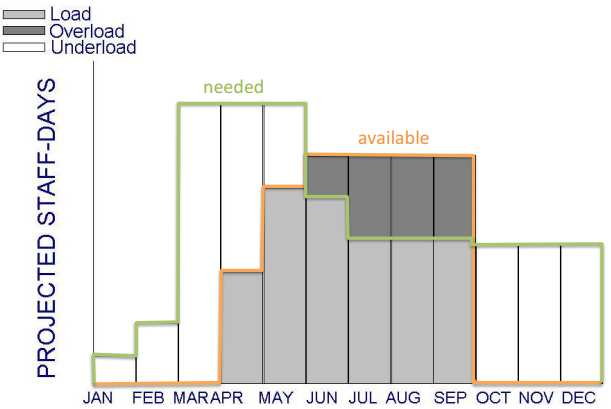
\includegraphics[width=0.5\linewidth]{resource_planning_and_tracking.png}
\end{tabular}

\subsubsection{Resource tracking}
Track the planed (resource usage) versus the actual (resource usage)

